% \documentclass[a4paper,10pt]{article}
% \usepackage[utf8]{inputenc}
% 
% %opening
% \title{}
% \author{}
% 
% \begin{document}
% 
% \maketitle

\section{Network-wide Allocation}
\paragraph{Single Switch}
% problem description
  We first extend CO2 to the case with single switch and multiple receivers. The topology of connection is shown in Figure {}. The switch holds rules with multiple action tag, and each action represents forwording the traffic to one receiver. The receivers feedback the top overselected IPs with regard to bytes volume to controller, and which rules to put into the Blacklist is decided by the controller. The challenge is that the Blacklist memory is a bottleneck. We propose a Q-Learning (RL) based Approach (QLA) in the controller to allocate constrainted Blacklist space to the rules with different actions.

    % System Combination
% Harish K Krishnamurthy <www.ece.neu.edu/~hkashyap/>
%\documentclass{article}

%\usepackage{tikz}
%\usetikzlibrary{shapes,arrows,shadows}
%\usepackage{amsmath,bm,times}
%\newcommand{\mx}[1]{\mathbf{\bm{#1}}} % Matrix command
%\newcommand{\vc}[1]{\mathbf{\bm{#1}}} % Vector command

%\begin{document}
% Define the layers to draw the diagram
\pgfdeclarelayer{background}
\pgfdeclarelayer{foreground}
\pgfsetlayers{background,main,foreground}

% Define block styles used later

\tikzstyle{sensor}=[draw, fill=blue!20, text width=4em, 
    text centered, minimum height=2.5em,drop shadow]
\tikzstyle{ann} = [above, text width=5em, text centered]
\tikzstyle{wa} = [sensor, text width=4em, fill=red!20, 
    minimum height=4em, rounded corners, drop shadow]
\tikzstyle{aggr} = [sensor, text width=6em, fill=red!20, 
    minimum height=4em, rounded corners, drop shadow]
\tikzstyle{sc} = [sensor, text width=13em, fill=red!20, 
    minimum height=10em, rounded corners, drop shadow]
    

% Define distances for bordering
\def\blockdist{3}
\def\edgedist{2.5}
\resizebox{1\linewidth}{!}{
\begin{tikzpicture}
    % draw one switch
    \node (wa) [wa]  {switch};
   
   % draw many receivers
    \path (wa.east)+(\blockdist,1) node (vote) [sensor] {Receiver1};
    \path (wa.east)+(\blockdist,0) node (vote1) [sensor] {Receiver2};
    \path (wa.east)+(\blockdist,-1) node (vote2) [sensor] {Receiver3};
    \path (wa.east)+(\blockdist,-2) node (vote3) [sensor] {Receiver4};
    

    % connect switch with receivers
    \path [draw, ->] (wa.east) -- node [above] {} 
        (vote.west);
    \path [draw, ->] (wa.east) -- node [above] {} 
        (vote1.west);
    \path [draw, ->] (wa.east) -- node [above] {} 
        (vote2.west);
    \path [draw, ->] (wa.east) -- node [above] {} 
        (vote3.west);     
    
    \begin{pgfonlayer}{background}
        \path (vote.north)+(1,0.3) node (ab) {};
        \path (vote.south)+(-1,-3.5) node (cb) {};
          
        \path[fill=yellow!20,rounded corners, draw=black!50, dashed]
            (ab) rectangle (cb);           
            
    \end{pgfonlayer}
    
 
    % connect Controller to Switch
    \path (wa.north)+(-3.7,0.2) node (ms) {};

\end{tikzpicture}
}

%\end{document}

% problem modeling
  Assume the system contains 1 switch and $n$ receivers, and we define a utility function $U_i$ for receiver $r$, we aim to maximize the following objective: % the objective should hightlight the target value
  
  $max \; \sum_{r = 1}^{n} U_r(a_{r,t})\;st.,$
  
  $\sum_{r = 1}^{n}a_{r,t} \leq A_c$
  
  Where $a_{r,t}$ is the Blacklist space allocated to the rules from receiver $r$ at time $t$, and $A_c$ is the Blacklist space capacity.
  
  We use reinforcement learning to compute the utility function for each receiver, so,
  
  $U_r(a_{r,t}) = Q_r(s_{r,t}, a_{r,t})$
  
  where function $Q_r$ is the value function in the reinforcement learning system, and $s_{r,t}$ is the state at time $t$.
% RL reinforcement learning
  
  Reinforcement learning is learning what to do-how to map situations to ations-so as to maximize a numerical reward signal[Reinforcement book]. Beyond the agent and the environment, one can identify four main subelements of a reinforcement learning system: a policy, a reward function, a value function, and optionally, a model of the environment[Reinforcement book]. 
  
  A policy defines the learning agent's way of behaving at a given time. A state $s_{r,t}$ in our design is the Blacklist space already allocated to the rules from receiver $r$, and a policy $a_{r,t}$ is to increase, decrease or maintain the allocation given on the current state. For example, policy 1 is to increase the allocation by 200 slots, and policy 2 is 100 slots decreament. 
  
  A reward function $r_t$ defines the goal in a reinforcement learning problem. We set a target overselection rate $ov_T$, and if the actual overselection rate $ov_a$ is larger than $ov_T$, the reward function is a negative scalar, otherwise, it is a positive scalar. By performing the reward function, we aim to control the actual overselection rate under or close to $ov_T$.
  
  We use Q-learning in our design, and the one-step Q-learning is defined by,
  
  $Q(s_t,a_t) \leftarrow Q(s_t,a_t) + \alpha \{r_{t+1})+\gamma\;max_{a}\;Q(s_{t+1},a)-Q(s_t,a_t)\}$
  
  The $Q_r(s_{r,t}, a_{r,t})$ value is kept at a table called Q table. There are $n$ tables for the $n$ reinforcement learning systems, respetively.
  
  The QLA is shown in procedural form in Algorithm{}.

  Initialize Q tables, policy and states. 
  
  Repeat (for each step of episode):
  
    foreach $s, s<m$
    
      foreach $r, r<n$
      
	Q-learning to update $Q_r(s_{r,t}, a_{r,t})$
	
      forend
      
    forend
    
  Repeat end
  
  
  Compute the maximum allocation from the $n$ tables by,
  
  $max \; \sum_{r = 1}^{n} U_r(a_{r,t})\;st.,$
  
  $\sum_{r = 1}^{n}a_{r,t} \leq A_c$
  
\paragraph{Multiple Switches}

  We extend our design to a network-wide case, with multiple switches and multiple receivers, and the topology of the switch and receivers is shown in Figure {}.. Assume the system contains $m$ switches, we define the objective function by,
  
  $max \; \sum_{s = 1}^{m}\sum_{r = 1}^{n} U_{s,r}(a_{s,r,t})\;st.,$
  
  $\sum_{r = 1}^{n}a_{s,r,t} \leq A_{c,s}$
  
  And,  
  
  $U_{s,r}(a_{s,r,t}) = Q_r(s_{s,r,t}, a_{s,r,t})$
  
  Where the subscript $s$ indicates switch $s$
  
  % System Combination
% Harish K Krishnamurthy <www.ece.neu.edu/~hkashyap/>
%\documentclass{article}

%\usepackage{tikz}
%\usetikzlibrary{shapes,arrows,shadows}
%\usepackage{amsmath,bm,times}
%\newcommand{\mx}[1]{\mathbf{\bm{#1}}} % Matrix command
%\newcommand{\vc}[1]{\mathbf{\bm{#1}}} % Vector command

%\begin{document}
% Define the layers to draw the diagram
\pgfdeclarelayer{background}
\pgfdeclarelayer{foreground}
\pgfsetlayers{background,main,foreground}

% Define block styles used later

\tikzstyle{sensor}=[draw, fill=blue!20, text width=4em, 
    text centered, minimum height=2.5em,drop shadow]
\tikzstyle{ann} = [above, text width=5em, text centered]
\tikzstyle{wa} = [sensor, text width=4em, fill=red!20, 
    minimum height=4em, rounded corners, drop shadow]
\tikzstyle{aggr} = [sensor, text width=6em, fill=red!20, 
    minimum height=4em, rounded corners, drop shadow]
\tikzstyle{sc} = [sensor, text width=13em, fill=red!20, 
    minimum height=10em, rounded corners, drop shadow]
    

% Define distances for bordering
\def\blockdist{3}
\def\edgedist{2.5}
\resizebox{1\linewidth}{!}{
\begin{tikzpicture}
    % draw multiple switches
    \node (wa) [wa]  {switch2};
    \path (wa.north)+(0,1) node (wa1) [wa] {switch1};
    \path (wa.south)+(0,-1) node (wa2) [wa] {switch3};
    \path (wa.south)+(0,-3) node (wa3) [wa] {...};
   
   % draw many receivers
    \path (wa.east)+(\blockdist,1) node (vote) [sensor] {Receiver1};
    \path (wa.east)+(\blockdist,0) node (vote1) [sensor] {Receiver2};
    \path (wa.east)+(\blockdist,-1) node (vote2) [sensor] {Receiver3};
    

    % connect switches with receivers
    \path [draw, ->] (wa.east) -- node [above] {} 
        (vote.west);
    \path [draw, ->] (wa.east) -- node [above] {} 
        (vote2.west);

        
    \path [draw, ->] (wa1.east) -- node [above] {} 
        (vote.west);
    \path [draw, ->] (wa1.east) -- node [above] {} 
        (vote1.west);
    \path [draw, ->] (wa2.east) -- node [above] {} 
        (vote2.west);
    \path [draw, ->] (wa3.east) -- node [above] {} 
        (vote2.west);

    
                
        
    
    \begin{pgfonlayer}{background}
        \path (vote.north)+(1,0.3) node (ab) {};
        \path (vote.south)+(-1,-3.5) node (cb) {};
          
        \path[fill=yellow!20,rounded corners, draw=black!50, dashed]
            (ab) rectangle (cb);           
            
    \end{pgfonlayer}
    
    
    
    
 
    % connect Controller to Switch
    \path (wa.north)+(-3.7,0.2) node (ms) {};

\end{tikzpicture}
}

%\end{document}
  
\paragraph{Experiment Settings}
 
\paragraph{Single Switch}
The receiver number $n = 4$ as shown in Figure{}, 

\begin{figure}[t!]
  \begin{center}
    \subfigure[The overselection rate]{\label{fig:aggrinterval_ov}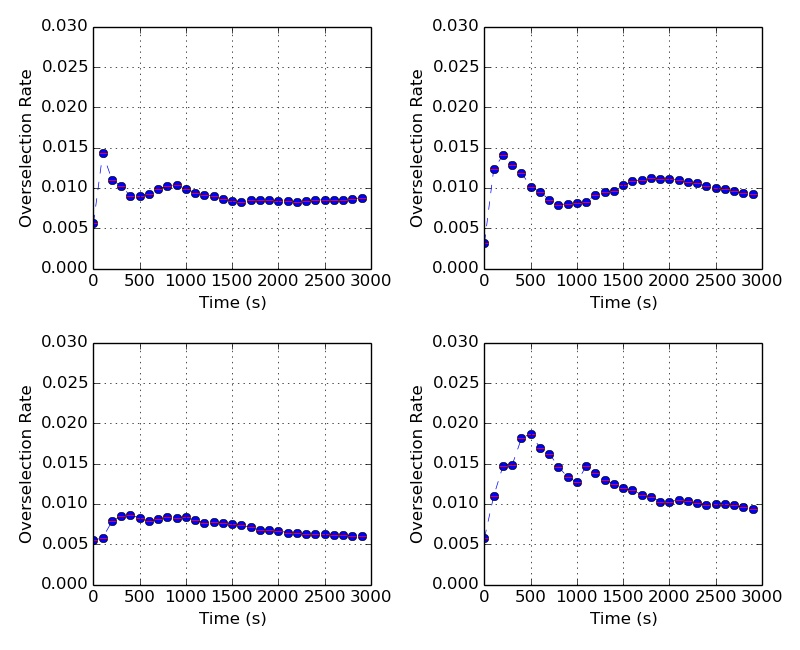
\includegraphics[width=0.5\textwidth]{figure/std_avg.jpg}}
    \subfigure[The convergence time]{\label{fig:aggrinterval_time}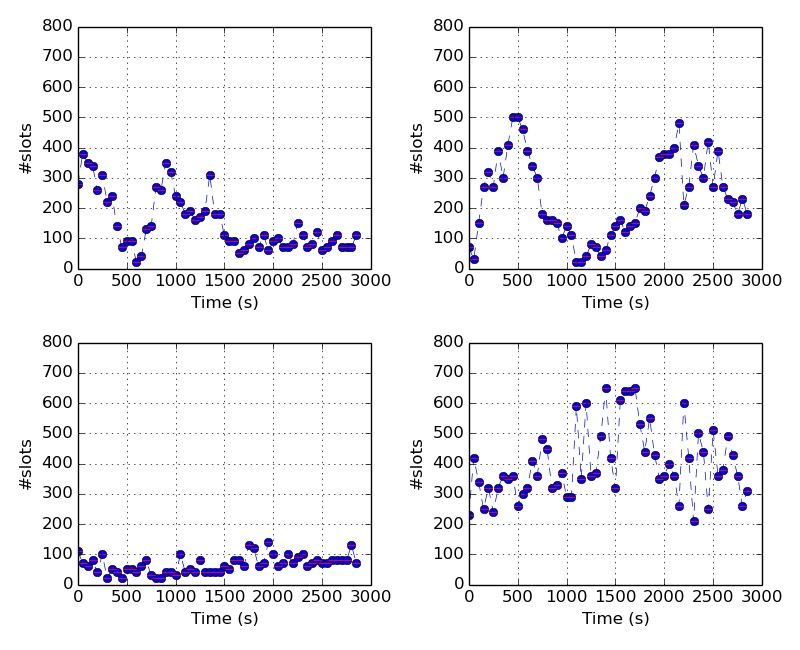
\includegraphics[width=0.5\textwidth]{figure/std_res.jpg}} \\
  \end{center}
  \caption{Results for different updating intervals for both the BUA and the DCA}
  \label{fig:aggrinterval}
\end{figure}


\paragraph{Multiple Switches}
The switch number $m = 3$, and the receiver number $n = 3$
  
\paragraph{Simulation Results and Analysis} 
  

% \end{document}
